\documentclass[12pt]{article}

\usepackage{fancyhdr}
\usepackage{amsthm}
\usepackage{amsmath}
\usepackage{graphicx}
\usepackage{amssymb}
\usepackage{esint}
\usepackage{subfigure}
\usepackage{color}
\usepackage{moreverb}
\usepackage{wrapfig}

\textwidth 17cm \topmargin -1cm \oddsidemargin 0cm \textheight 21.5cm
\pagestyle{empty} \pagestyle{fancyplain}
\lhead[\fancyplain{}{}]{\fancyplain{}{{\sc Adam Farnsworth:}}}
\chead[\fancyplain{}{}]{\fancyplain{}{{\sc Midterm}}}
\rhead[\fancyplain{}{}]{\fancyplain{}{{\sc Fall 2017}}}

\newcommand{\etal}{\textit{et al. }}

\begin{document}
\centerline{\Large\textbf{Midterm}}
\vspace{2cm}

\section*{Introduction}\label{sec::Intro}
The goal of this project is to study the motion of a spinning soccer ball.  It will be kicked over a wall in the hopes of curving the trajectory to deceive the opponent, and ultimately making it into the goal.  The set up will have the feild in a three dimensional plane with x,y and z coordinates.  The x-axis goes parallel to the goal line, the y-axis points towards the center of the field and the z-axis points upwards, while the origin is in the center of the goal.  Denote as $(x^0, y^0, z^0)$ the initial  location of the ball and as $(v_x^0,v_y^0,v_z^0)$ is velocity right after the strike.  Three forces influence the ball trajectory: the gravitational force, the drag force due to the air resistance and the lift force due to the Magnus effect. According to Newton’s second law the motion of the ball in this situation is described by the equation
 \begin{eqnarray}
m\overrightarrow{a} = m\overrightarrow{g} - c_{drag}|v|\overrightarrow{v} + c_{lift}|v|\overrightarrow{s}X\overrightarrow{v}\\\nonumber
       \end{eqnarray}
where $\overrightarrow{a},\overrightarrow{v},\overrightarrow{s}$ are vectors representing x,y,z for acceleration, velocity, and spin direction.  $m = 0.437$kg, $\overrightarrow{g}$ is gravity at $9.81\frac{m}{s}$, $c_{drag}$ is drag at 0.0057, and $c_{lift}$ is magnus effect at 0.0061
Taking Newton's second  law of motion, I put it into a system of equations for x,y and z as seen below:
\begin{center}
$\begin{cases} 
m\frac{d^2x}{dt^2} = -c_{drag}|v|v_x+c_{lift}|v|(s_yv_z-s_zv_y)  \\
m\frac{d^2y}{dt^2} =-c_{drag}|v|v_y+c_{lift}|v|(s_zv_x-s_xv_z)\\ 
m\frac{d^2z}{dt^2} = -mg-c_{drag}|v|v_z+c_{lift}|v|(s_xv_y-s_yv_x)
 \end{cases}$
\end{center}
where $|v| = \sqrt{v_x^2+v_y^2+v_z^2}$ and $v_x = \frac{dx}{dt},v_y = \frac{dy}{dt},v_z= \frac{dz}{dt}$\\
The starting position and velocity of the ball constitute initial conditions for the system
\begin{center}
$\begin{cases}
x(0) = x^0, y(0) = y^0, z(0) = z^0 \\
\frac{dx}{dt}(0) =v_x^0,\frac{dy}{dt}(0) = v_y^0,\frac{dz}{dt}(0) = v_z^0,\\
 \end{cases}$
\end{center}


\newpage
\section{Problem 1}\label{sec::Problem 1}
Question:\\
Write system of equations from above as a system of first-order ODEs\\
\\
Given the initial conditions for the starting position $x(0) = x^0, y(0) = y^0, z(0) = z^0$ and velocity $\frac{dx}{dt}(0) =v_x^0,\frac{dy}{dt}(0) = v_y^0,\frac{dz}{dt}(0) = v_z^0$ the system of equations can be solved as a first-order ODE.  If we keep velocity $\frac{dx}{dt} =v_x,\frac{dy}{dt} = v_y,\frac{dz}{dt} = v_z$ as a unknown function we can rewrite the system of equations in the form:
\begin{center}
$\begin{cases}
\frac{dx}{dt} = v_x \\ 
\frac{dy}{dt} = v_y \\ 
\frac{dz}{dt} = v_z \\ 
\frac{dv_x}{dt} =\frac{ -c_{drag}|v|v_x+c_{lift}|v|(s_yv_z-s_zv_y)}{m}  \\
\frac{dv_y}{dt} =\frac{-c_{drag}|v|v_y+c_{lift}|v|(s_zv_x-s_xv_z)}{m}\\ 
\frac{dv_z}{dt} = \frac{-mg-c_{drag}|v|v_z+c_{lift}|v|(s_xv_y-s_yv_x)}{m}
 \end{cases}$
\end{center}
While initial conditions become:
\begin{center}
$\begin{cases}
x(0) = x^0, y(0) = y^0, z(0) = z^0 \\
v_x(0) =v_x^0,v_y(0) = v_y^0,v_z(0) = v_z^0,\\
 \end{cases}$
\end{center}
These equations form a system of first-order ODEs!

\newpage
\section{Problem 2}\label{sec::Problem 2}
Question:\\
Write a MATLAB function for solving a general system of first-order ODEs of size m using the fourth-order accurate Runge-Kutta Method (RK4).\\
\\The function is of the form: $[t, y] = solveode(f, y0, t_{start}, t_{final}, dt)$\\
First I find the size of the arrays, preallocate arrays for the return values t and y, and put initial values into the return arrays.  Then I loop through all the cases while checking for overshooting from dt.  During this loop I calculate the new time, calculate all values for the RK4 formula, and then add the value to y.\\
\\A general system of m first-order differential equations can be written as
\begin{center}
$\begin{cases} 
\frac{dy^{(1)}}{dt} = f^{(1)}(t,y^{(1)},...,y^{(m)})  \\
\frac{dy^{(2)}}{dt} = f^{(2)}(t,y^{(1)},...,y^{(m)})  \\
\vdots \\
\frac{dy^{(m)}}{dt} = f^{(m)}(t,y^{(1)},...,y^{(m)})  \\
 \end{cases}$
\end{center}
with initial conditions:
\begin{center}
$\begin{cases} 
y^{(1)}(t_0) = y_0^{(1)} \\
y^{(2)}(t_0) = y_0^{(2)} \\
\vdots \\
y^{(m)}(t_0) = y_0^{(m)} \\
 \end{cases}$
\end{center}
where $y^{(1)}(t),y^{(2)}(t), ... , y^{(m)}(t)$ are unknown solutions, $f^{(1)}, f^{(2)}, ... , f^{(m)}$ are given functions of $m+1$ variables, $t_0$ is the given initial time and $y_0^{(1)},y_0^{(2)}, ... , y_0^{(m)}$ are initial values of the unknown functions.  This system can be written in a much shorter way using the vector notation. I denote $\overrightarrow{y},\overrightarrow{y}_0, \overrightarrow{f}$ by the following vectors:
\begin{eqnarray}
   \overrightarrow{y}= \begin{bmatrix}
           y^{(1)}(t) \\
          y^{(2)}(t) \\
           \vdots \\
           y^{(m)}(t)
         \end{bmatrix},
 \overrightarrow{y}_0= \begin{bmatrix}
           y_0^{(1)} \\
          y_0^{(2)} \\
           \vdots \\
           y_0^{(m)}
         \end{bmatrix},
 \overrightarrow{f}= \begin{bmatrix}
           f^{(1)}(t,y^{(1)}, ... , y^{(m)}) \\
           f^{(2)}(t,y^{(1)}, ... , y^{(m)}) \\
           \vdots \\
           f^{(m)}(t,y^{(1)}, ... , y^{(m)}) \\
         \end{bmatrix}
\end{eqnarray}


The classical fourth-order accurate Runge-Kutta method (RK4) for systems of ODEs is given by:
\begin{eqnarray}
 \overrightarrow{y}_{n+1}= \overrightarrow{y}_n+\Delta t (\frac{\overrightarrow{k}_1+2\overrightarrow{k}_2+2\overrightarrow{k}_3+\overrightarrow{k}_4}{6})\\\nonumber
\end{eqnarray}
 where the slopes $\overrightarrow{k}_1, \overrightarrow{k}_2, \overrightarrow{k}_3, \overrightarrow{k}_4$ are computed as
\begin{eqnarray} 
\overrightarrow{k}_1 &=& \overrightarrow{f}(t_n, \overrightarrow{y}_n) \\\nonumber
\overrightarrow{k}_2 &=&  \overrightarrow{f}(t_n+.5 \Delta t, \overrightarrow{y}_n + .5 \Delta t \overrightarrow{k}_1) \\\nonumber
\overrightarrow{k}_3 &=&  \overrightarrow{f}(t_n+.5 \Delta t, \overrightarrow{y}_n + .5 \Delta t \overrightarrow{k}_2) \\\nonumber
\overrightarrow{k}_4 &=&  \overrightarrow{f}(t_n+\Delta t, \overrightarrow{y}_n + \Delta t \overrightarrow{k}_3) \\\nonumber
 \end{eqnarray}


\newpage
\section{Problem 3}\label{sec::Problem 3}
Question:\\
Test your MATLAB function using the system of equations
\begin{center}
$\begin{cases} 
m\frac{ dy^{(1)} }{dt} =y^{(2)}  \\
m\frac{ dy^{(2)} }{dt} =sin(1-exp(y^{(2)} )) \\
m\frac{ dy^{(3)} }{dt} =\frac{1}{1-ln(y^{(5)}-1)}  \\
m\frac{ dy^{(4)} }{dt} =(\frac{1}{2}t^2 + t)y_2 + exp(y^{(3)})y^{(1)}  \\
m\frac{ dy^{(5)} }{dt} =1-y^{(5)}  \\
m\frac{ dy^{(6)} }{dt} =-3(\frac{exp(y^{(3)})-1}{1+t^3})^2  \\
 \end{cases}$
\end{center}
with initial conditions\\
\begin{center}
$y^{(1)}(0)=0, y^{(2)}(0)=0, y^{(3)}(0)=0, y^{(4)}(0)=0, y^{(5}(0)=2, y^{(6)}(0)=1$
\end{center}
The exact solution to this test problem is
\begin{center}
$\begin{cases} 
y_{exact}^{(1)}(t) = sin(t)  \\
y_{exact}^{(2)}(t) = cos(t)  \\
y_{exact}^{(3)}(t) = ln(1+t)  \\
y_{exact}^{(4)}(t) = (\frac{1}{2}t^2 _ t)sin(t)  \\
y_{exact}^{(5)}(t) = 1 + exp(-t)  \\
y_{exact}^{(6)}(t) = \frac{1}{1+t^3}  \\
 \end{cases}$
\end{center}
Take $t_{start} = 0, t_{final} = 1$. Compute the order of accuracy using time-steps\\ $\Delta t = 0.1, 0.05, 0.025, 0.0125, 0.00625$ and make sure that your ODE solver produces the expected order of accuracy.

\begin{table}[bht]
\centering

\begin{tabular}{|l|l|l|}
\hline
dt      & error        & order of accuracy \\ \hline
0.1 & 1.243384e-06 & 3.91220           \\ \hline
0.05 & 8.258789e-08  & 3.95172          \\ \hline
0.025 &5.337419e-09  &3.97425           \\ \hline
0.0125 &3.395953e-10  & 3.98668           \\ \hline
0.00625 & 2.142154e-11 & 3.99231           \\ \hline

\end{tabular}
\caption{Problem 3 solutions}
\label{problem 3}
\end{table}



\newpage
\section{Problem 4}\label{sec::Problem 4}
Question:\\
Use your function to solve the system of equations describing the motion of a spinning ball and
obtain trajectories of the ball for each of the cases presented in Table 2 (in all cases $c_{drag} = 0.0057,
c_{lift} = 0.0061, h_{wall} = 2$). Take $t_{start} = 0, t_{final} = 2$ and $\Delta t = 0.02$.
\begin{table}[bht]
\centering

\begin{tabular}{|l|l|l|l|l|l|l|l|l|l|l|l|l|l|}
\hline
\multicolumn{1}{|r|}{} & \multicolumn{3}{l|}{Location} & \multicolumn{3}{l|}{Velocity} & \multicolumn{3}{l|}{Spin} & \multicolumn{4}{l|}{Wall}                                                     \\ \hline
case no.               & $x^0$    & $y^0$    & $z^0$   & $v_x^0$  & $v_y^0$  & $v_z^0$ & $s_x$   & $s_y$  & $s_z$  & $x_{start}^{wall}$ & $y_{start}^{wall}$ & $x_{end}^{wall}$ & $y_{end}^{wall}$ \\ \hline
1                      & −15      & 23       & 0       & 18       & −23      & 8.5     & 0.10    & 0.10   & -0.99   & −11.2              & 14.7               & −8.6             & 16.0             \\ \hline
2                      & 25.5     & 15       & 0       & −28      & −11      & 7.5     & 0       & 0      & 1      & 18.1               & 9.7                & 17               & 11.3             \\ \hline
3                      & −4       & 35       & 0       & −8       & −36      & 5       & −0.32   & 0      & 0.95   & −4.3               & 25.9               & −0.8             & 25.9             \\ \hline
4                      & 16       & 28       & 0       & −25      & −20      & 8       & 0.10    & 0.15   & 0.98   & 12.6               & 19.6               & 9.9              & 20.8             \\ \hline
\end{tabular}
\caption{Direct free kick examples}
\label{Table 1:}
\end{table}

\begin{figure}[h]
\centering    
\subfigure[case no. 1]{\label{fig:a}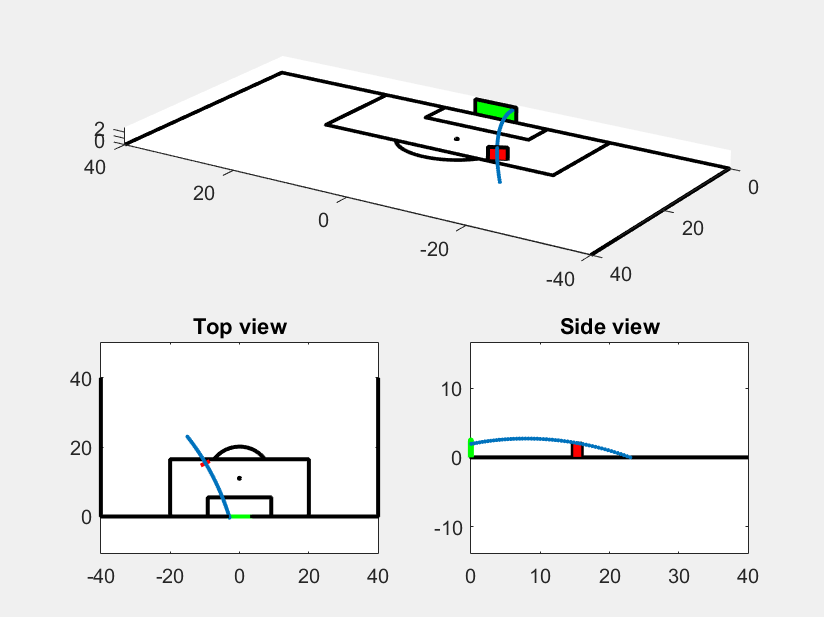
\includegraphics[width=60mm]{1}}
\subfigure[case no. 2]{\label{fig:b}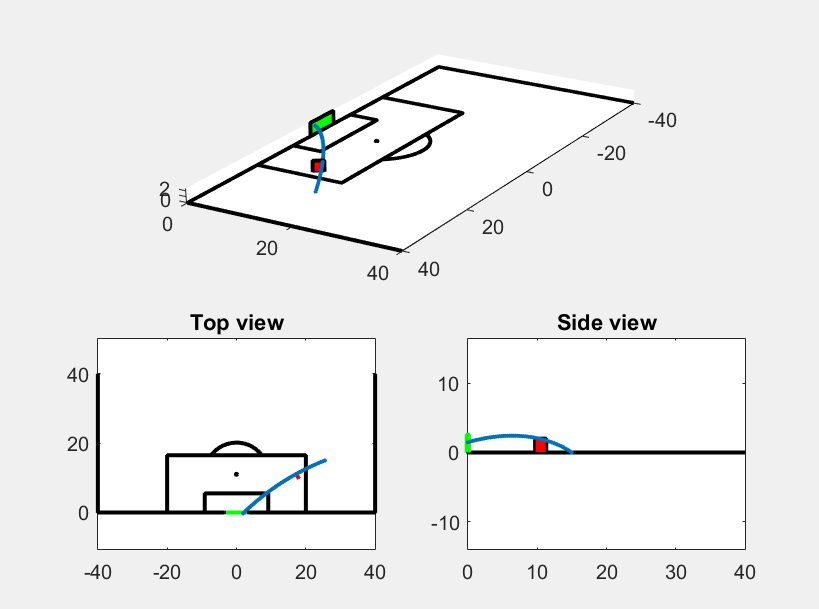
\includegraphics[width=60mm]{2}}
\subfigure[case no. 3]{\label{fig:a}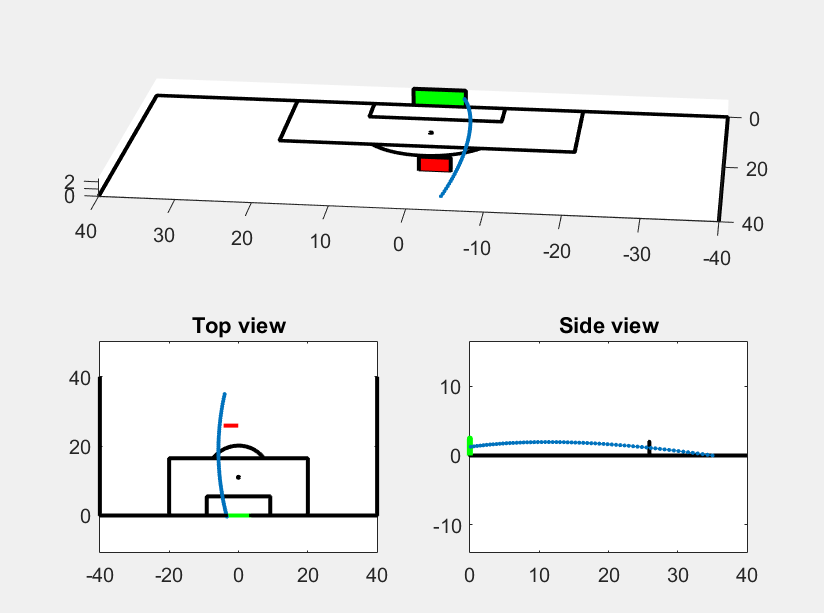
\includegraphics[width=60mm]{3}}
\subfigure[case no. 4]{\label{fig:b}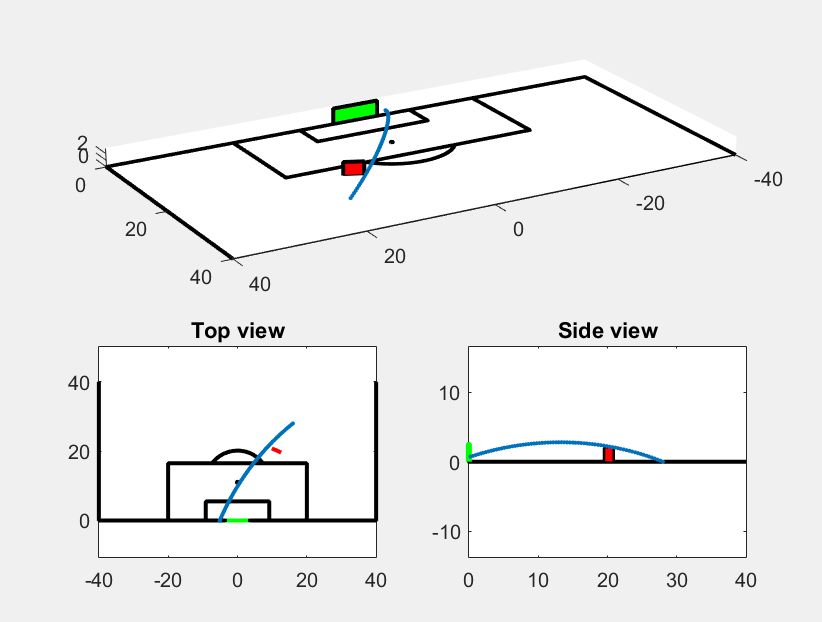
\includegraphics[width=60mm]{4}}
\caption{Direct free kick plots}
\end{figure}




\newpage
\section{Problem 5}\label{sec::Problem 5}
Question:\\
Write a code that analyzes the trajectories of the ball and determines whether the ball hits the
defensive wall and whether the ball goes into the goal. Determine the outcome of the free kick
for each of the cases in Table 2.\\
\\
Solutions:\\
Case number 1 made it over wall and made the goal.\\
Case number 2 hit wall, but if it made it past it would of made the goal.\\
Case number 3 made it over wall and made the goal.\\
Case number 4 made it over wall and missed the goal.\\
\\
How I figured this out:\\
1) Find trajectory of the 3 arrays : x, y, z\\
2) Analyze trajectory by either checking if it went into goal or hit the wall.  To do this for the goal I checked if 2 points (line) pass the plane of the goal.  To find the n, I found where $y(n)>0, y(n+1)<0$ which is when the path of the ball crosses the goal.  This is because it gives us the y coordinate  before crossing (n) and after (n+1).  From there the equation below represents finding the time ($t^*$) when y crosses the goal, followed by the reduction to get $t^*$ alone:
\begin{eqnarray}
y &=& y_n + (t^* - t_n)\frac{y_{n+1}-y_n}{t_{n+1}-t_n}=0\\\nonumber
t^* &=& -y_n\frac{t_{n+1}-t_n}{y_{n+1}-y_n} + t_n \\\nonumber
\end{eqnarray}
The x and z coordinates at this time will be represented by $x^*, z^*$.  to find these I will take the time found above and use them in the following equations:
\begin{eqnarray}
x^* &=& x_n + (t^* - t_n)\frac{x_{n+1}-x_n}{t_{n+1}-t_n}\\\nonumber
z^* &=& z_n + (t^* - t_n)\frac{z_{n+1}-z_n}{t_{n+1}-t_n}\\\nonumber
\end{eqnarray}
Now that I have the cordinates, I can check if they are within the bounds of the goal.  If they are, the ball made it into the goal!\\
\\
The logic to check if the ball hit the wall is similar to checking the goal.  This time instead of the y coordinate passing at 0, its a bit more involved.  The following equation shows the y coordinate at the wall.
\begin{eqnarray}
y = y_s^w + (x - x_s^w)\frac{y_e^w-y_s^w}{x_e^w-x_s^w}\\\nonumber
\end{eqnarray}
where $x_s^w, x_e^w, y_s^w, y_e^w$ are x coordinate at the start of wall, x coordinate at the end of wall, y coordinate at the start of wall, y coordinate at the end of wall respectively.  Similarly  to checking the goal, I need to find the n where the path of the ball crosses the goal.  To find use the equations below finding n:
\begin{eqnarray}
y_{n} > y_s^w + (x_n - x_s^w)\frac{y_e^w-y_s^w}{x_e^w-x_s^w}\\\nonumber
y_{n+1} < y_s^w + (x_{n+1} - x_s^w)\frac{y_e^w-y_s^w}{x_e^w-x_s^w}\\\nonumber
\end{eqnarray}
This is because it gives us the y coordinate before crossing (n) and after (n+1).\\
From this n we can use it to find the x,y and z coordinates which will be represented by $x^*,y^*,z^*$.  To start out we have 2 equations for $y^*$, and we can set them to be equal to each other in order to find $x^*$.
\begin{eqnarray}
 y_n + (x^* - x_n)\frac{y_{n+1}-y_n}{x_{n+1}-x_n}=y_s^w + (x^* - x_s^w)\frac{y_e^w-y_s^w}{x_e^w-x_s^w}\\\nonumber
\end{eqnarray}
After isolating $x^*$ I am left with the equation:
\begin{eqnarray}
x^* = \frac{y_s^w - y_n + x_n\frac{y_{n+1}-y_n}{x_{n+1}-x_n}- x_s^w\frac{y_e^w-y_s^w}{x_e^w-x_s^w}}{\frac{y_{n+1}-y_n}{x_{n+1}-x_n}-\frac{y_e^w-y_s^w}{x_e^w-x_s^w}}\\\nonumber
\end{eqnarray}
Now that I have a solution for $x^*$ I can solve for $y^*,z^*$ with the equations below:
\begin{eqnarray}
y^* =  y_n + (x^* - x_n)\frac{y_{n+1}-y_n}{x_{n+1}-x_n} \\\nonumber
z^* =  z_n + (x^* - x_n)\frac{z_{n+1}-z_n}{x_{n+1}-x_n} \\\nonumber
\end{eqnarray}
From here I check if $x^*,y^*,z^*$ is within the bounds of the wall.

%%%%%%%%%%%
\newpage
\clearpage
\setcounter{page}{1} \pagestyle{empty}
\section{References}\label{sec::References}
\begin{itemize}
\item [1] Daniil Bochkov, CS 111 - Introduction to Computational Science midterm Fall 2017
\item [2] Daniil Bochkov, CS 111 - Introduction to Computational Science Lecture 4 High-order Methods 2017
\item [3] Daniil Bochkov, CS 111 - Introduction to Computational Science Lecture 6 Systems of ODEs 2017
\item [4] Daniil Bochkov, CS 111 - Introduction to Computational Science Lecture 7 High-Order ODEs 2017
\end{itemize}


%%%%%%%%%%%

\end{document}
